\chapter{Segway Presentation}
In the following chapter, an overview of how a segway works is presented. This includes a block description of the system, and a description of the functionalities	 it is to have.
The segway provided by Aalborg University is also described, in regards to the mechanical frame and the provided hardware.

\section{Generalized Segway Description}
A segway can be seen as a typical control system, as shown in \autoref{fig:seg_over}.
Here, the controlled parameters are acquired using various transducers, processed by the system controller and then a control signal is outputted to the actuator(s) through. Apart from the control system, a \gls{RC} is added to the system, which can also be seen in \autoref{fig:seg_over}. The reason for this will be described later on. In the case of the segway, the transducers are sensors, providing information on the movement of the segway, and the actuators are motors, which are driving the wheels. 

\begin{figure}[H]
\centering
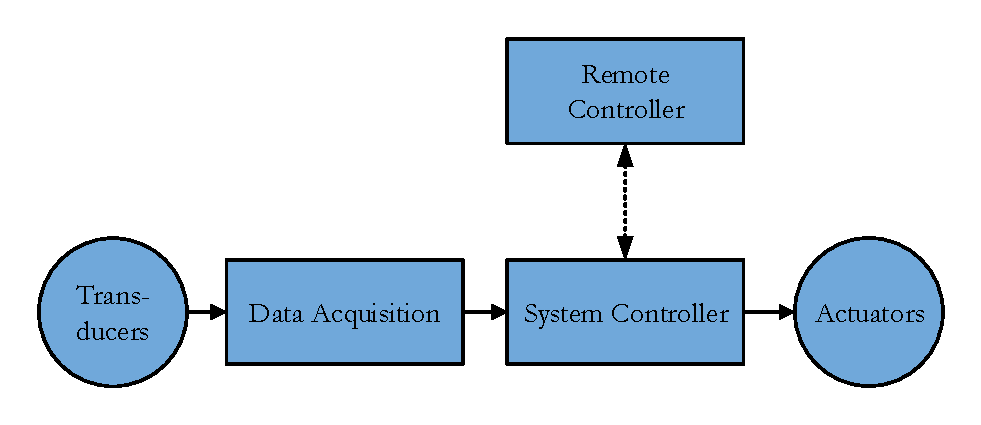
\includegraphics[width=0.7\textwidth]{figures/segwayOverview.pdf}
\caption{Generalized block diagram of a segway control system.}
\label{fig:seg_over}
\end{figure}

It is decided that the segway is to have four main functionalities to function as desired. These functionalities are \textit{balancing, driving, turning and the ability to be remote controlled}. Each of these are described in further detail in the following section.

\subsection{Functionalities of the System Controller}
The controller unit has four main functionalities, namely balancing, driving, turning, and transceiving wireless signals between the \gls{RC} and the system controller. Each of these functionalities are described in further detail in the following section.

One of the required functionalities of any segway is the ability to balance. The system controller must control the motors so the inverted pendulum is balancing vertically. Because the pendulum is unstable by nature, the controller has to make the system stable. This functionality relies on input from the transducers, which is used to calculate an actuator signal to keep the segway balanced.

%The movement and control of the system can be based of the current state of the segway measured by transducers. The transducers can for example tell about the current position, speed, and acceleration of the segway. 

%The data will then be processed in the microcontroller which determines how the segway should react to the current state.

%\subsubsection{Transceiving of wireless commands}
Through a wireless RC the segway is remote controlled. This means that the segway must be capable of receiving commands from the RC and make the segway move accordingly. To achieve this, the segway and RC must share a communication protocol. The wireless RC should also able to receive information regarding the movement of the segway like the speed, angular velocity and angle.

%\subsubsection{Driving and turning}
The driving and turning functionalities are responsible for controlling the segway's forward and backwards velocity as well as the direction of the segway. To ensure the segway does not fall over when driving or turning, the movement will of course have to happen in corporation with the balancing functionality, since balance is still to be kept when driving and turning.

%The velocity of the segway can be controlled by changing which angle the balance functionality tries to uphold. To keep this new angle, the balance functionality must respond to the change in angle, by changing the translatoric velocity. In other words, the rotational moment must be countered by an equal translatoric force.

%Unlike the driving functionality, the turning functionality does not lead to changes in the balance functionality, since turning is rotation around a different axis.

%These functionalities are in the same control unit as they must correlate with the balance functionality, since the output of both the balance, driving and turning functionalities must be merged before it is sent to the motor control unit.
